% PRL look and style (easy on the eyes)
\documentclass[aps,pre,twocolumn,nofootinbib,superscriptaddress,linenumbers]{revtex4-1}
% Two-column style (for submission/review/editing)
%\documentclass[aps,prl,preprint,nofootinbib,superscriptaddress,linenumbers]{revtex4-1}

\pdfoutput=1
\usepackage[pdftex]{graphicx}

\usepackage{alltt}

%\usepackage{palatino}

%\usepackage{palatino}
% Change to a sans serif font.
\usepackage{sourcesanspro}
\renewcommand*\familydefault{\sfdefault} %% Only if the base font of the document is to be sans serif
\usepackage[T1]{fontenc}
%\usepackage[font=sf,justification=justified]{caption}
\usepackage[font=sf]{floatrow}

% Rework captions to use sans serif font.
\makeatletter
\renewcommand\@make@capt@title[2]{%
 \@ifx@empty\float@link{\@firstofone}{\expandafter\href\expandafter{\float@link}}%
  {\sf\textbf{#1}}\sf\@caption@fignum@sep#2\quad
}%
\makeatother

\usepackage{listings} % For code examples
\usepackage[usenames,dvipsnames,svgnames,table]{xcolor}

% Break URLs in bibliography correctly
%\usepackage{biblatex}
%\usepackage{url}
%\setcounter{biburllcpenalty}{7000}
%\setcounter{biburlucpenalty}{8000}

\usepackage{amsmath}
\usepackage{amssymb}
%\usepackage[mathbf,mathcal]{euler}
%\usepackage{citesort}
\usepackage[caption=false]{subfig}
\usepackage{dcolumn}
\usepackage{boxedminipage}
\usepackage{verbatim}
\usepackage{url}
\def\UrlBreaks{\do\/\do-}
\usepackage{breakurl}
\usepackage[breaklinks,colorlinks=true,citecolor=blue,linkcolor=blue]{hyperref}
\usepackage[group-separator={,}]{siunitx}

%Strikethrough
\usepackage[normalem]{ulem}

% Justification
\captionsetup{singlelinecheck=off}

% Pretty-printing of shell commands
\newcommand{\shellcmd}[1]{\\\ \texttt{\scriptsize #1}}

% The figures are in a figures/ subdirectory.
\graphicspath{{../figures/}}

%% DOCUMENT %%%%%%%%%%%%%%%%%%%%%%%%%%%%%%%%%%%%%%%%%%%%%%%%%%%%%%%%%%%%%%%%%%%%
\begin{document}

%% TITLE %%%%%%%%%%%%%%%%%%%%%%%%%%%%%%%%%%%%%%%%%%%%%%%%%%%%%%%%%%%%%%%%%%%%
\title{Modeling error in experimental assays using the bootstrap principle:\\
Understanding discrepancies between assays using different dispensing technologies}

\author{Sonya M. Hanson}
  \affiliation{Computational Biology Program, Sloan Kettering Institute, Memorial Sloan Kettering Cancer Center, New York, NY 10065, United States}
\author{Sean Ekins}
  \affiliation{Collaborations in Chemistry, Fuquay-Varina, NC 27526, United States}
\author{John D. Chodera}
 \thanks{Corresponding author}
 \email{john.chodera@choderalab.org}
  \affiliation{Computational Biology Program, Sloan Kettering Institute, Memorial Sloan Kettering Cancer Center, New York, NY 10065, United States}

\date{\today}

%%%%%%%%%%%%%%%%%%%%%%%%%%%%%%%%%%%%%%%%%%%%%%%%%%%%%%%%%%%%%%%%%%%%%%%%%%%%%%%%%%%%%%%%%%%%%%%%%%%%%%
% ABSTRACT/pacs
%%%%%%%%%%%%%%%%%%%%%%%%%%%%%%%%%%%%%%%%%%%%%%%%%%%%%%%%%%%%%%%%%%%%%%%%%%%%%%%%%%%%%%%%%%%%%%%%%%%%%%
\begin{abstract}

All experimental assay data contains error, but the magnitude, type, and primary origin of this error is often not obvious.
Here, we describe a simple set of assay modeling techniques based on the bootstrap principle that allow sources of error and bias to be simulated and propagated into assay results.
We demonstrate how deceptively simple operations---such as the creation of a dilution series with a robotic liquid handler---can significantly amplify imprecision and even contribute substantially to bias.
To illustrate these techniques, we review an example of how the choice of dispensing technology can impact assay measurements, and show how the primary contributions to discrepancies between assays can be easily understood and potentially corrected for.
These simple modeling techniques---illustrated with an accompanying IPython notebook---can allow modelers to understand the expected error and bias in experimental datasets, and even help experimentalists design assays to more effectively reach accuracy and imprecision goals.

\end{abstract}

\maketitle

%%%%%%%%%%%%%%%%%%%%%%%%%%%%%%%%%%%%%%%%%%%%%%%%%%%%%%%%%%%%%%%%%%%%%%%%%%%%%%%%%%%%%%%%%%%%%%%%%%%%%%
% INTRODUCTION
%%%%%%%%%%%%%%%%%%%%%%%%%%%%%%%%%%%%%%%%%%%%%%%%%%%%%%%%%%%%%%%%%%%%%%%%%%%%%%%%%%%%%%%%%%%%%%%%%%%%%%
\section{Introduction}
\label{section:introduction}

Measuring the activity and potency of ligands---whether in biophysical or cell-based assays---is an important tool in the understanding of biological processes.
However, understanding assay data for the purpose of optimizing small molecules for use as chemical probes or potential therapeutics is complicated by the fact that all assay data are contaminated with error from numerous sources.

Often, the dominant contributions to assay error are simply not known.
This is unsurprising, given the number and variety of potential contributing factors.
Even for what might be considered a straightforward assay involving fluorescent measurements of a ligand binding to a protein target, this might include (but is by no means limited to): compound impurities and degradation~\cite{kozikowski_effect_2003,kozikowski_effect_2003-1,cheng_studies_2003,waybright_overcoming_2009}, imprecise compound dispensing  ~\cite{harris_gradient_2010,grant_achieving_2009}, unmonitored water absorption by DMSO stocks ~\cite{waybright_overcoming_2009}, the effect of DMSO on protein stability~\cite{tjernberg_dmso-related_2005}, intrinsic compound fluorescence~\cite{simeonov_fluorescence_2008,baell_new_2010}, compound insolubility~\cite{di_biological_2006} or aggregation~\cite{mcgovern_common_2002,mcgovern_kinase_2003,feng_high-throughput_2005,feng_synergy_2006,baell_new_2010}, variability in protein concentration or quality, pipetting errors, and inherent noise in any fluorescence measurement---not to mention stray lab coat fibers as fluorescent contaminants~\cite{busch_does_2015}. 
Under ideal circumstances, control experiments would be performed to measure the magnitude of these effects, and data quality tests would either reject flawed data or ensure that all contributions to error have been carefully accounted for in producing an assessment of error and confidence for each assayed value.

Unfortunately, by the time the data reach the hands of a computational chemist (or other data consumer), the opportunity to perform these careful control experiments has long passed.
In the worst case, the communicated assay data may not contain any estimate of error at all. 
Even when error has been estimated, it is often not based on a holistic picture of specific information known about the assay.
% JDC: I might tinker with the next few sentences to make it clear that this "analysis of heterogeneous public data" is a prior of last resort.
One approach that has been useful is aggregating many datasets to give a crude estimate of the general reliability of a similar set of assays by quantifying the variation in measurements of a single quantity~\cite{kramer_experimental_2012,kalliokoski_comparability_2013}. 
Care must be taken to distinguish between fully independent replicates and partial replicates that only repeat part of the experiment (for example, repeated measurements performed using the same stock solutions), since partial measurements can often underestimate true error by orders of magnitude~\cite{chodera_entropy-enthalpy_2013}.
Alternatively, when multiple independent measurements are not available, the knowledge of how a particular assay was conducted can inform the construction of an assay-specific model incorporating some of the dominant contributions to error in a manner that can be highly informative.

Here, we review some common sources of error in experimental assays, and describe a set of simple modeling concepts based on the bootstrap principle.
Using only the assay protocol and basic specifications of the imprecision and inaccuracy of various operations such as weighing and volume transfers, we show how to construct and simulate a simple model of the assay that incorporates these important (often dominant) sources of error. 
This approach, while simple, provides a powerful tool to understand how assay error depends on both the assay protocol and the imprecision and inaccuracy of basic operations, as well as the true value of the quantity being measured (such as compound affinity). 
This strategy is not limited to computational chemists and consumers of assay data---it can be also used to help optimize assay formats before an experiment is performed, help troubleshoot problematic assays after the fact, or ensure that all major sources of error are accounted for by checking that variation among control measurements match expectations.

We illustrate these concepts by considering a recent example from the literature: a report by Ekins et al.~\cite{ekins_dispensing_2013} on how the choice of dispensing technology impacts the apparent biological activity of the same set of compounds under otherwise identical conditions.
The datasets employed in the analyses~\cite{barlaam_novel_2009,barlaam_pyrimidine_2010} were originally generated by AstraZeneca using either a standard liquid handler with fixed (washable) tips or an acoustic droplet dispensing device to prepare the assay, resulting in highly divergent assay results (Figure~\ref{fig:overview}).
The assay probed the effectiveness of a set of pyrimidine compounds as anti-cancer therapeutics, targeting the EphB4 receptor, thought to be a promising target for several cancer types~\cite{xia_ephb4_2005,bardelle_inhibitors_2008}.
While the frustration for computational modelers was particularly great, since quantitative structure activity relationship (QSAR) models derived from these otherwise identical assays produce surprisingly divergent predictions, numerous practitioners from all corners of drug discovery expressed their frustration in ensuing blog posts and commentaries~\cite{lowe_drug_2015,evanko_serial_2013,ekins_what_2013}.
Hosts of potential reasons were speculated, including sticky compounds absorbed by tips ~\cite{palmgren_drug_2006} and compound aggregation ~\cite{feng_synergy_2006,feng_high-throughput_2005}.

%We make use of this real-world example to illustrate some of the basic concepts behind modeling the most common sources of error in assays.
For simplicity, we ask whether the simplest contributions to assay error---imprecision and bias in material transfer operations and imprecision in measurement---might account for some component of the discrepancy between assay techniques.
We make use of basic information---the assay protocol as described (with some additional inferences based on fundamental concepts such as compound solubility limits) and manufacturer specifications for imprecision and bias---to construct a model of each dispensing process to determine the overall inaccuracy and imprecision of the assay as a function of true compound affinity, and identify the steps that contribute the most to these assay data errors.
To better illustrate these techniques, we also provide an annotated IPython notebook [\url{http://choderalab.org/dispensing-errors-manuscript}] that includes all of the computations described here in detail.
Readers are encouraged to download these notebooks and explore them to see how different assay configurations affect assay error, and potentially customize the notebooks for their own scenarios.

\begin{figure*}[tb]
   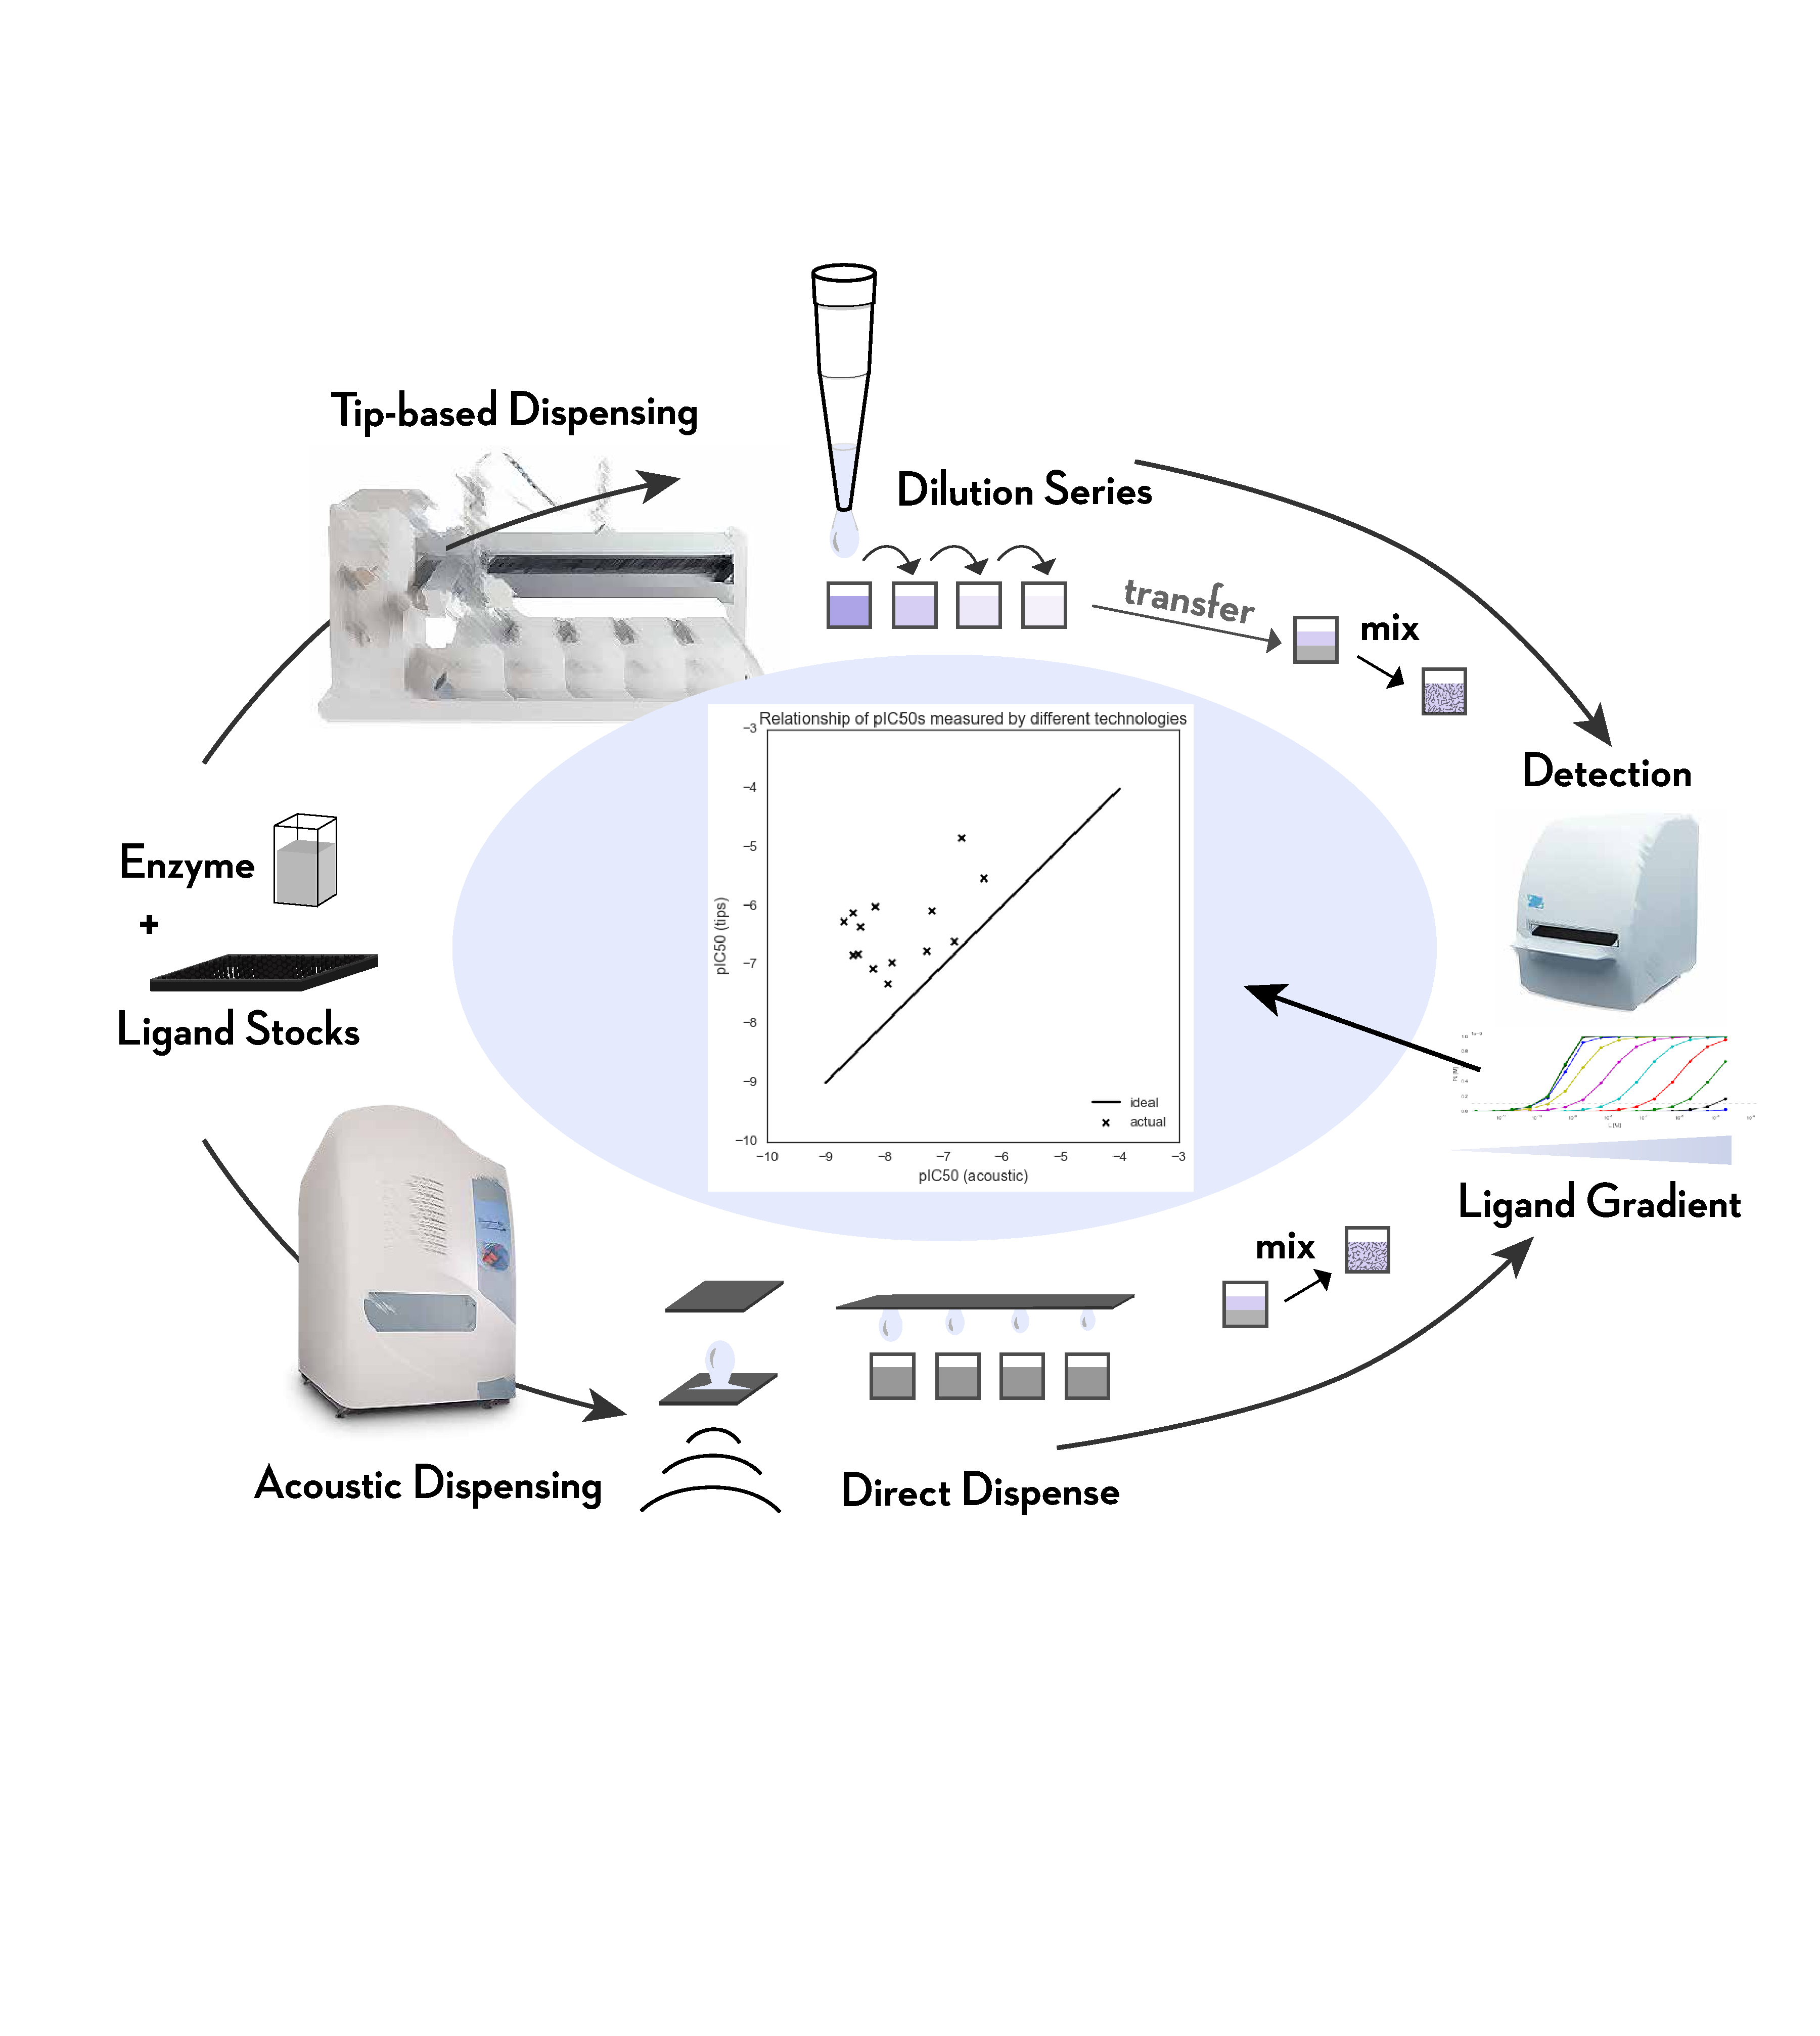
\includegraphics[trim={0 15cm 0 8cm},clip,width=0.75\textwidth]{../figures/Fig1-4.pdf}
  \caption{{\bf Illustration of the stages of the two assay protocols considered here, for both tip-based and acoustic dispensing.}
  Two different assay protocols---utilizing different dispensing technologies---were used to perform the same assay discussed in \citep{ekins_dispensing_2013}.
  In the case of tip-based dispensing, a Tecan Genesis liquid handler was used to create a serial dilution from which the final assay mixture was prepared. 
  In the case of acoustic dispensing, a LabCyte Echo was used to directly dispense different amounts of compound into the assay mixture.
  Product accumulation was measured for various concentrations of ligand with the same concentration of protein, and the resulting data were fit to obtain pIC$_{50}$ estimates.
  The resulting pIC$_{50}$ data for each assay protocol were highly discrepant, as shown in the central figure plotting the two against each other.
   }
  \label{fig:overview}
\end{figure*}


%%%%%%%%%%%%%%%%%%%%%%%%%%%%%%%%%%%%%%%%%%%%%%%%%%%%%%%%%%%%%%%%%%%%%%%%%%%%%%%%%%%%%%%%%%%%%%%%%%%%%
% Experimental error
%%%%%%%%%%%%%%%%%%%%%%%%%%%%%%%%%%%%%%%%%%%%%%%%%%%%%%%%%%%%%%%%%%%%%%%%%%%%%%%%%%%%%%%%%%%%%%%%%%%%%
\section{Experimental error}

Overall experimental error can be broken into two components: The \emph{imprecision} (quantified by standard deviation or variance), which characterizes the random component of the error that causes different replicates of the same assay to give slightly different results, and the \emph{inaccuracy} (quantified by bias), which is the deviation of the average over many replicates from the true value of the quantity being measured.

There are a variety of sources of experimental error. 
Random variation in the quantity of liquid delivered by a pipette, random errors in the reported mass of a dry compound, or random errors in the measured fluorescence of a well will all contribute to the imprecision of an assay measurement.
The important thing is that the mean of these errors over many repetitions is zero. 
If the mean is \emph{not} zero, this is an example of inaccuracy, or bias---where a calibration error leads to a systematic deviation in the volume delivered by a pipette, the mass measured by a balance, or the average fluorescence measured by a plate reader.

\section*{Modeling experimental error}

There are many approaches to the modeling of error and its propagation into derived data.
Often, undergraduate laboratory courses provide an introduction to the tracking of measurement imprecision, demonstrating how to propagate imprecision in individual measurements into derived quantities using Taylor series expansions---commonly referred to simply as \emph{propagation of error}~\cite{taylor_introduction_1997}.
For example, for a function $f(x,y)$ of two measured quantities $x$ and $y$ with associated errors $\sigma_x$ and $\sigma_y$, the first-order Taylor series error propagation rule is,
\begin{eqnarray}
\delta^2 f &=& \left[\frac{\partial f}{\partial x}\right]^2_x \, \sigma^2_x + \left[\frac{\partial f}{\partial y}\right]^2_y \sigma^2_y + \left[\frac{\partial f}{\partial x}\right]_x \left[\frac{\partial f}{\partial y}\right]_y \, \sigma^2_{xy} \nonumber \\ \label{equation:error-propagation}
\end{eqnarray}
where the correlated error $\sigma^2_{xy} = 0$ if the measurements of $x$ and $y$ are independent.

For addition or subtraction of two independent quantities, this rule gives a simple, well-known expression for the additivity of errors in quadrature,
\begin{eqnarray}
f(x,y) &=& x \pm y \nonumber \\
\delta^2 f &=& \sigma^2_x + \sigma^2_y 
\end{eqnarray}
For more complex functions of the data, however, even the simple form of Eq.~\ref{equation:error-propagation} for just two variables is a struggle to apply.

Instead, we adopt a different approach based on the \emph{bootstrap principle}~\cite{shalizi_simple_????}.
\emph{Bootstrapping} allows you to approximate the sampling distribution by simulating from a good estimate (or simulacrum) of the real process.
While many computational chemists may be familiar with \emph{resampling bootstrapping} for a large dataset, where resampling from the dataset with replacement provides this estimate of the real process, it is also possible to simulate the process in other ways, such as from a parametric or other model of the process.
Here, we model sources of random error using simple statistical distributions, and \emph{simulate} multiple replicates of the experiment, examining the distribution of experimental outcomes to quantify error.
Unlike propagation of error based on Taylor series (Eq.~\ref{equation:error-propagation}), quantifying approach by boostrap simulation is straightforward even for the most complex assays.
In fact, practical application of the bootstrap principle doesn't even require that the function $f$ be differentiable or even something that can be written down easily in closed form---as long as we can compute the function $f$ on a dataset, we can bootstrap it.

For example, for the case of  quantities $x$ and $y$ and associated errors $\sigma_x$ and $\sigma_y$, we would conduct many realizations $n = 1, \ldots, N$ of an experiment in which we draw \emph{bootstrap replicates} $x_n$ and $y_n$ from normal (Gaussian) distributions
\begin{eqnarray}
x_n &\sim& \mathcal{N}(x, \sigma^2_x) \nonumber \\
y_n &\sim& \mathcal{N}(y, \sigma^2_y) \nonumber \\
f_n &\equiv& f(x_n, y_n)
\end{eqnarray}
and then analyze the statistics of the $\{f_n\}$ samples as if we had actually run the experiment many times.
For example, we can quantify the statistical uncertainty $\delta f$ using the standard deviation over the bootstrap simulation realizations, $\mathrm{std}(f_n)$.
Alternatively, presuming we have simulated enough bootstrap replicates, we can estimate 68\% or 95\% confidence intervals, which may sometimes be very lopsided if the function $f$ is very lopsided.

Since most instruments we deal with in a laboratory---such as pipettes or liquid handlers or balances---have manufacturer specifications for imprecision and accuracy, we will generally make use of the normal (Gaussian) distribution\footnote{Volumes, masses, and concentrations must all be positive, so it is more appropriate in principle to use a \emph{lognormal} distribution to model these processes to prevent negative values.  In practice, however, if the relative imprecision is relatively small and negative numbers do not cause large problems for the functions, a normal distribution is sufficient.} in these error models,
\begin{eqnarray}
x \sim \mathcal{N}(\mu, \sigma^2) \label{equation:Gaussian}
\end{eqnarray}
where the mean $\mu$ represents the inaccuracy and standard deviation $\sigma$ the imprecision, with $\sigma^2$ being the variance of the normal distribution.

We will generally quantify the error from our bootstrap simulation replicates in terms of two primary statistics:
\begin{description}
\item[Bias] As a measure of inaccuracy, we will compute the mean deviation from the true value,
\begin{eqnarray}
\mathrm{bias} &\equiv& E[ f_n - f ]
\end{eqnarray}
where $E[\cdot]$ is the expectation, the average over many bootstrap replicates.
\item[Coefficient of variation (CV)] As a measure of imprecision, we will compute the relative standard deviation,
\begin{eqnarray}
\mathrm{CV} &\equiv& \frac{\mathrm{std}(f_n)}{E[f_n]}
\end{eqnarray}
\end{description}
which we represent here as a percent, rather than a fraction.

%Here, we take the approach that it is as simple as adding known values for imprecision and inaccuracy in pipetting into a model of your assay, and using parametric bootstrapping [ref] to sample through many replicates and getting a resulting expected bias and coefficient of variation (CV), which correspond to the imprecision and inaccuracy, respectively. 

% JDC: I reorganized the material a bit, but feel free to work some of this text into the above if I left out anything important!
%\subsection*{Error propagation}
%
%Error propagation, for example when we have many pipetting steps in a row each with its own error, can be a bit trickier to implement. 
%While there are a variety of ways of doing this, derivable from the Taylor Expansion, using parametric bootstrapping [ref] to sample through many replicates, as mentioned above, avoids having to implement these more complex forms of error propagation.
%Bootstrapping allows you to approximate the sampling distribution by simulating from a good estimate of the real process.
%The more common form of boostrapping is resampling bootstrapping, where the 'good estimate of the real process' resamples estimates from the observed sample.
%Here, parametric bootstrapping is used, where the 'good estimate of the real process' is a simulation of a model.
%This works well for a variety of models, and here we show it for a specific rather simple case, but it can be expanded to include much more complicated error models, without making the math of the error propagation any more complicated.
%In this case knowing the sampling distribution lets us quantify uncertainty

\subsection*{Simple liquid handling: Mixing solutions}

Consider the simplest kind of liquid transfer operation, in which we use some sort of pipetting instrument (handheld or automated) to combine two solutions.
For simplicity, we presume we combine a volume $V$ of compound stock solution of known true concentration $C$ with a quantity of buffer of volume $W$.
We presume, again for simplicity, that these operations are free of bias, but have associated imprecisions $\sigma_V$ and $\sigma_W$. 
These imprecisions might come from stated manufacturer specifications in the absence of other calibration information.

To simulate this process, we simply simulate a number of realizations $n = 1, \ldots, N$, where we again assume a normal distribution for the sources of uncertainty,
\begin{eqnarray}
v_n &\sim& \mathcal{N}(V, \sigma_V^2) \nonumber \\
w_n &\sim& \mathcal{N}(W, \sigma_W^2) \nonumber \\
c_n &=& C / (v_n + w_n)
\end{eqnarray}
and then compute statistics for the $\{c_n\}$, $n = 1,\ldots,N$ that are produced by this process.
To compute the bias, we know that we \emph{expect} the resulting concentration $c = C/ (V + W)$.

We can further extend this model to include uncertainty $\sigma_C$ in the stock concentration $C$, and begin to see how powerful and modular the bootstrap scheme is.
In this new model, each simulation realization $n$ consists of
\begin{eqnarray}
C_n &\sim& \mathcal{N}(C, \sigma_C^2) \nonumber \\
v_n &\sim& \mathcal{N}(V, \sigma_V^2) \nonumber \\
w_n &\sim& \mathcal{N}(W, \sigma_W^2) \nonumber \\
c_n &=& C_n / (v_n + w_n)
\end{eqnarray}
All we had to do was add one additional step to our bootstrap simulation scheme in which the stock concentration $C_n$ is drawn from a normal distribution with each bootstrap realization.
The model can be expanded indefinitely with additional independent measurements or random variables in the same simple way.

Below, we exploit this modularity to design a simple scheme to simulate an entire assay without being overwhelmed by complexity.
All of the errors we discuss arise  from the transfer and mixing of volumes of solutions with different concentrations of compound as described above.
While the completeness of mixing can itself be a source of error in certain assays---a surprising amount of effort is required to ensure thorough mixing~\cite{walling_mixing_2007,weiss_modeling_2002,mitre_turbo-mixing_2007}---we have chosen not to explicitly include this incomplete mixing effect in our model, but it could similarly be added within this framework.
Next, we will use this method of modeling error and apply it to a specific example from the literature, looking at IC$_{50}$s for compounds targeting the EphB4 receptor~\cite{ekins_dispensing_2013,barlaam_novel_2009,barlaam_pyrimidine_2010}, breaking down how errors differ depending on the dispensing technology under otherwise identical conditions.

\subsection*{Modeling an enzymatic reaction}

The EphB4 assay~\cite{ekins_dispensing_2013,barlaam_novel_2009,barlaam_pyrimidine_2010} measures the accumulation of phosphorylated substrate over some short interval of time when the inhibitor is added in different concentrations in the presence of substrate; fitting a curve obtained over a range of inhibitor concentrations yields an observed IC$_{50}$.

A simple model for this competition assay can be created using standard models for competitive inhibition of a substrate $S$ with an inhibitor $I$ to compute a quantity that will be related to this measurement. 
Here, we assume the total accumulation of product in a fixed assay time will be proportion to the relative enzyme turnover velocity $V_0 / V_\mathrm{max}$, and use an equation derived assuming Michaelis-Menten kinetics,
\begin{eqnarray}
\frac{V_{0}}{V_\mathrm{max}} = \frac{[S]}{K_{m}(1+\frac{[I]}{K_{i}})+[S]} \label{equation:competitive-inhibition} ,
\end{eqnarray}
where the Michaelis constant $K_{m}$ and substrate concentration $[S]$ for the EphB4 system are pulled directly from the assay methodology description~\cite{barlaam_novel_2009,barlaam_pyrimidine_2010}.
Note that what is observed in the experiment is actually product accumulation, which is modeled by the velocity times time, $V_0 t$, assuming that there is an excess of substrate, and here we just report this relative to the uninhibited enzyme---$(V_0 t) / (V_\mathrm{max} t) = V_0 / V_\mathrm{max}$.
In interrogating our model, we will vary the true inhibitor affinity $K_{i}$ to determine how the assay imprecision and inaccuracy depend on true inhibitor affinity.
Thus the activity, $V_{0}/V_{max}$, depends only on the inhibitor concentration $[I]$, which we compute statistics for exactly as defined for $c_n$ above.

\subsection*{Advanced liquid handling: Making a dilution series}

Because the affinities and activities of compounds can vary across a dynamic range that spans several orders of magnitude, it is common for assays to utilize a dilution series of some sort to measure the activity and potency of ligands. 
To create a dilution series, an initial compound stock is diluted into buffer in the first well of the series, and the contents mixed; for each subsequent well, a volume from the previous well combined with buffer and mixed (Figure~\ref{fig:dilution}).
Commonly, each subsequent dilution step uses fixed ratios, such as 1:1 or 1:10 of dilution:buffer.

It is easy to see how a dilution series can amplify sources of error:
because each dilution step involves multiple pipetting operations, and the previously prepared dilution in the series is used to prepare the next dilution, errors will grow with each dilution in the series.
As a result, the instrumentation used can have a substantial impact on the results obtained.
Here we compare an aqueous dilution series made with a tip-based liquid handler (specifically the Tecan Genesis), and a direct-dispensing dilution series made with acoustic dispensing (specifically the Labcyte Echo).

\subsubsection*{Tip-based liquid handling}

To create a serial dilution series (Figure~\ref{fig:dilution}), we start with an initial well at concentration $C_\mathrm{initial}$ and sequentially transfer volume $V_\mathrm{transfer}$ into a volume $V_\mathrm{buffer}$ of buffer in the next well and mix, repeating this process $n_\mathrm{dilutions}$-1 times to create a total of $n_\mathrm{dilutions}$ dilutions. 
To model the impact of imprecision and inaccuracy on this process, we use manufacturer-provided specifications\footnote{While manufacturer-provided specifications for imprecision and inaccuracy are often presented as the maximum-allowable values, we find these are a reasonable starting point for this kind of modeling.} for the Tecan Genesis: the relative imprecision is stated to be 3\% and the inaccuracy as 3-5\% for the volumes in question~\cite{_tecan_2001}. 
The resulting concentration of each dilution operation is determined by both the concentration $C_{n-1}$ of the previous dilution step, which accumulates error with each dilution $n$, and by the pipetted volumes $V_\mathrm{transfer}$ and $V_\mathrm{buffer}$, each of which is randomly drawn from a normal distribution.
\begin{eqnarray}
\color{red}
\mathrm{[EQUATIONS]}
\end{eqnarray}
{\color{red}[JDC: We should express what a step of the dilution series looks like in terms of the equations for drawing random numbers as in the above sections.]}
Here, we estimate the bias and the variance using a linear interpolation of the provided imprecision and inaccuracy values in the manufacturer-provided table~\cite{_tecan_2001}.
Then, applying the parametric bootstrapping model, which is simply sampling over this variation with many replicates, we can get a good estimate for the errors in volumes and concentrations (Figure~\ref{fig:volumes-n-concentrations}).
Furthermore, as can be seen in the schematic in Figure~\ref{fig:overview}, because the dilution series is created before addition of the compound to the enzyme solution, there is an additional error term added upon transferring the dilution series results into the enzyme solution (in this case 2 $\mu$L into 10 $\mu$L).

\begin{figure}[tb]
    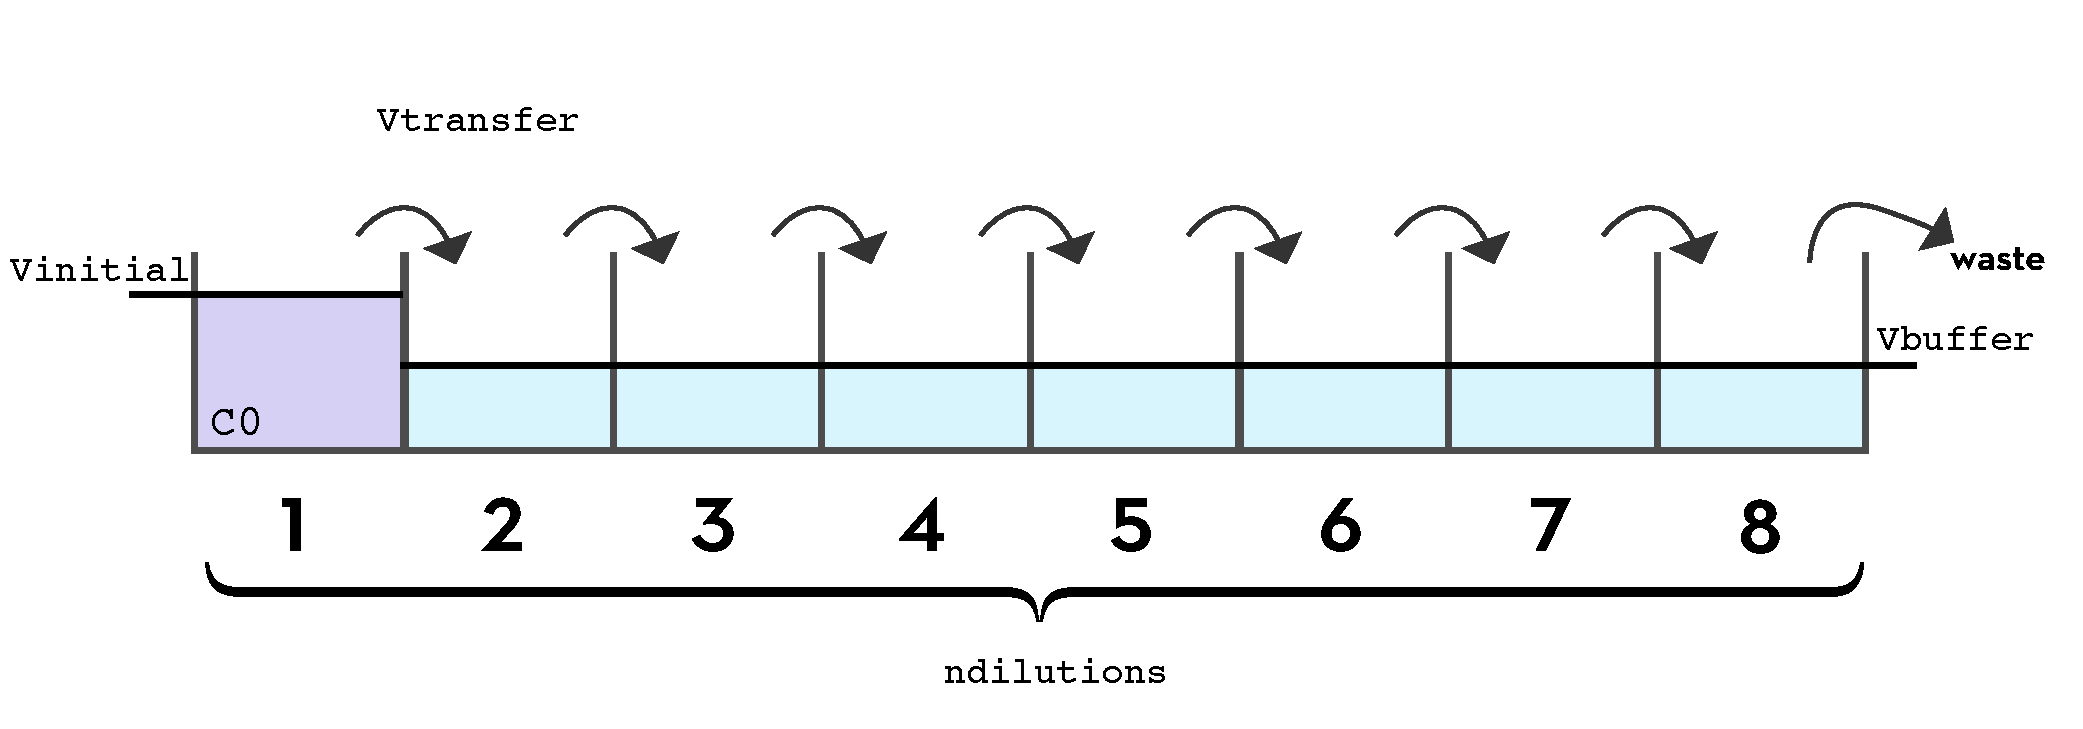
\includegraphics[width=\columnwidth]{../figures/dilution.pdf}

  \caption{{\bf A programmatic tip-based dilution series.}
  In this dilution series we start with our initial well at concentration, $C_\mathrm{intial}$, with initial volume, $V_\mathrm{initial}$. 
  A volume of the previous dilution, $V_\mathrm{transfer}$, is then transferred into a volume of buffer, $V_\mathrm{buffer}$. 
  In the case of a 1:1 dilution series, $V_\mathrm{transfer}$ and $V_\mathrm{buffer}$ are equal, so the intended concentration in the second well will be $C_\mathrm{initial}/2$. 
  This transfer is then repeated for all subsequent wells to create a total of $n_\mathrm{dilutions}$ dilutions. 
  For convenience, we assume that a volume $V_\mathrm{transfer}$ is removed from the last well so that all wells have the same final volume of $V_\mathrm{transfer} = V_\mathrm{buffer}$.
  }
  \label{fig:dilution}
\end{figure}

\subsubsection*{Direct dispensing technologies}

To construct a model of a dilution series, we start with our initial ligand stock in DMSO at concentration $C_0$ and transfer a volume $dispense\_volume$ into each well (Figure~\ref{fig:direct_dispense}). 
We can add imprecision and bias to this by using manufacturer-provided values.
For the Labcyte Echo, the imprecision is stated as 8\% and the inaccuracy as 10\% for the volumes in question~\cite{_echo_2011}. 
The concentration of each well is determined by the volumes $dispense\_volume$ and $mix\_volume$, each of which is defined in our model as randomly drawn from a normal distribution, where the bias and the variance that have been pulled from a linear interpolation of the provided imprecision and inaccuracy, respectively, provided by the manufacturer.
\begin{eqnarray}
\color{red}
\mathrm{[EQUATIONS]}
\end{eqnarray}
{\color{red}[JDC: We should express what a step of the dilution series looks like in terms of the equations for drawing random numbers as in the above sections.]}
We can then produce an estimate for the errors in volumes and concentrations (Figure~\ref{fig:volumes-n-concentrations}) by applying our parametric bootstrap model, generating many synthetic replicates of the experiment.
Because direct dispensing technologies dispense directly into the enzyme assay, rather than creating an intermediate dilution series that is then transferred into the assay wells, direct dispensing experiments include fewer steps (and hence fewer potential inaccuracy- and imprecision-amplifying steps) than the tip-based assays which must create the intermediate dilution series.

\begin{figure}[tb]
    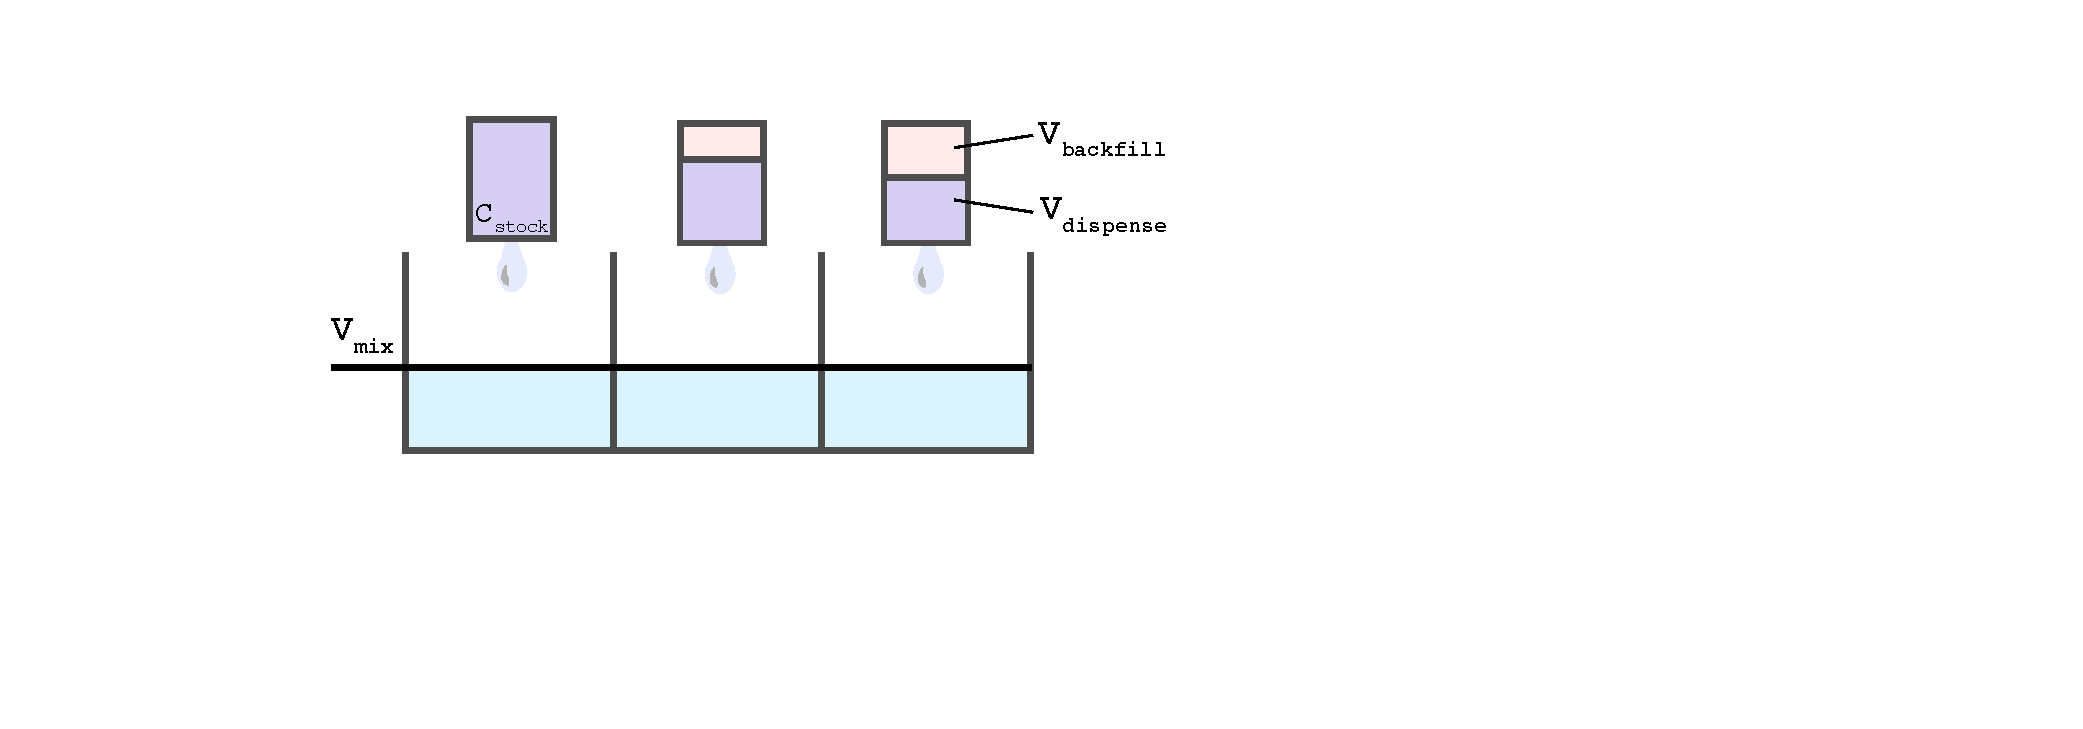
\includegraphics[trim={0 9cm 0 9cm},clip,width=\columnwidth]{../figures/direct_dispense.pdf}

  \caption{{\bf A programmatic direct dispense-based dilution series.}
  With direct dispense, each well is defined individually, not depending on the other, and $C_0$ defines the concentration of the ligand stock. 
  The $mix\_volume$ defines the final volume of the enzyme and ligand mix. 
  The $dispense\_volume$ is the amount of the compound stock in DMSO that is dispensed into the $mix\_volume$, and is what determines the final concentration of the ligand in the direct dispense assay setup. 
  To maintain a constant DMSO concentration throughout the assay, in this case 120 nL, a volume, defined by $backfill\_volume$, of pure DMSO is dispensed into the assay.
  }
  \label{fig:direct_dispense}
\end{figure}

\subsubsection*{Fixed tips and the dilution effect}

Simply including the computed contributions from inaccuracy and imprecision in our model of the  Ekins.~et al.~dataset~\cite{ekins_dispensing_2013}, it is easy to see that the imprecision is not nearly large enough to explain the discrepancies between measurements made with the two dispensing technologies~(Figure~\ref{fig:IC50_bias}).
Another aspect of dispensing with multichannel liquid-handler, specific to liquid-based fixed-tip pipetting, such as the Tecan Genesis has, is the dilution effect. 
This dilution effect was previously characterized by two papers from Bristol Myers Squibb~\cite{dong_use_2006,gu_dilution_2007}, where they found that the system liquid used to create the pressure differences required for pipetting, can mix with sample when it is being aspirated (Figure~\ref{fig:dilution_effect}). 
This mix of system liquid and sample dilutes the sample, and the Bristol Myers Squibb team was able to use a combination of the Artel dye-based Multichannel Verification System (MVS) and gravimetric methods to quantify that this dilution contributes a -6.30\% inaccuracy for a target volume of 20 $\mu$L~\cite{dong_use_2006}.
This inaccuracy can then be included in an expanded version of our original bootstrap model, and we can look at the resulting CV and bias seen in volumes, concentrations and quantities, as for the disposable tip model (which won't have this error) and the acoustic-dispensing model (Figure~\ref{fig:volumes-n-concentrations}).
This extra dilution effect also needs to be incorporated into the transfer of the dilution series into the enzyme assay solution, and it turns out this additional error is non-trivial.

\begin{figure}[tb]
   % 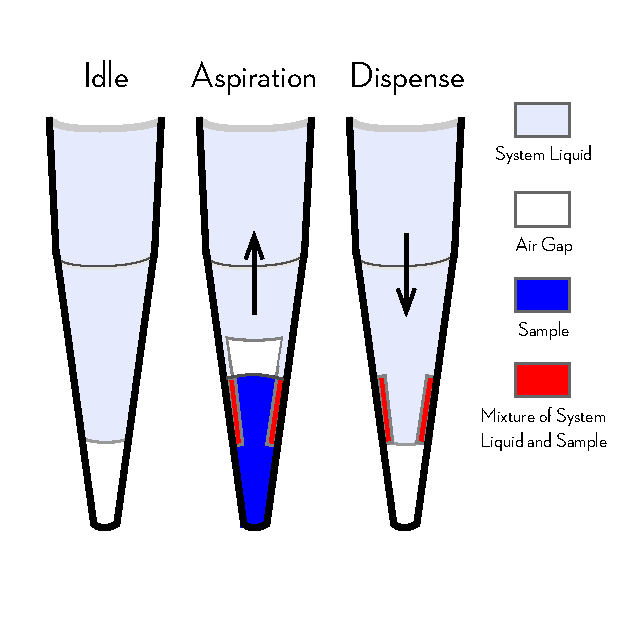
\includegraphics[width=0.325\textwidth]{../figures/dilution_effect.pdf}
    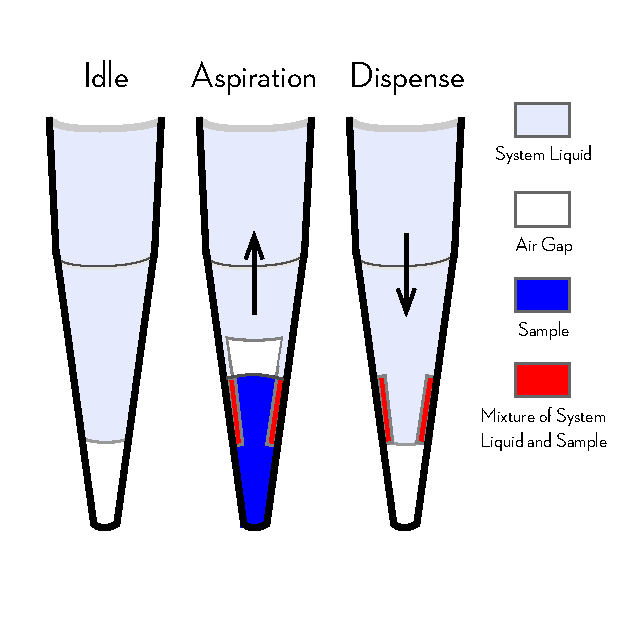
\includegraphics[width=\columnwidth]{../figures/dilution_effect.pdf}

  \caption{{\bf Fixed tips dilute aspirated samples with system liquid.}
  Automated liquid handlers with fixed tips utilizing liquid-displacement pipetting technology use a washing cycle in which system liquid (generally water or buffer) purges samples from the tips in between liquid transfer steps.
  Aspirated sample (blue) can be diluted by the system liquid (light purple) when some residual system liquid remains wetting the inside walls of the tip after purging.
  This residual system liquid is mixed with the sample as it is aspirated, creating a mixture of system liquid and sample (red) that dilutes the sample that is dispensed. 
  While the use of an air gap (white) reduces the magnitude of this dilution effect, dilution is a known issue in fixed tip liquid-based automated liquid handling technologies, requiring more complex liquid-handling strategies to eliminate it~\cite{gu_dilution_2007}. 
  Diagram adapted from Ref.~\cite{gu_dilution_2007}. 
  }
  \label{fig:dilution_effect}
\end{figure}


\begin{figure*}[tb]
    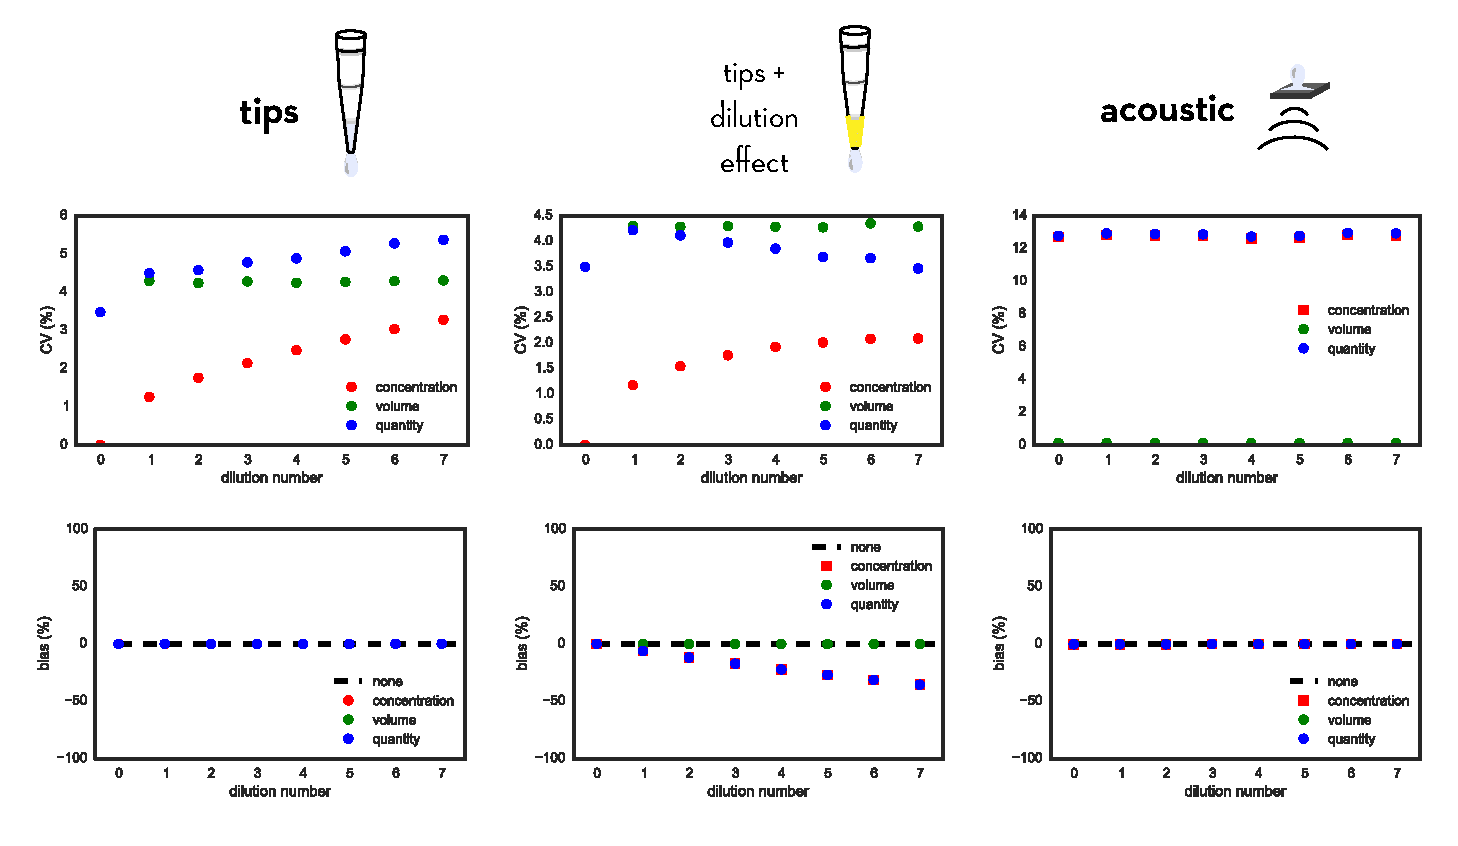
\includegraphics[width=1.0\textwidth]{../figures/volumes-n-concentrations.pdf}

  \caption{{\bf Modeled accumulation of random and systematic error in creating dilution series with fixed tips and acoustic dispensing.}
  The model predicts how errors in compound concentration, well volume, and compound quantity accumulate for a dilution series prepared using fixed tips neglecting dilution effects (\emph{left}) or including dilution effects (\emph{middle}) compared with an acoustic direct-dispensing process (\emph{right}).
  Imprecision and inaccuracy parameters appropriate for a Tecan Genesis (fixed tips dispensing) or LabCyte Echo (acoustic dispensing) were used, and assume that the initial compound stocks had negligible concentration error; see text for more details.
  The top panels show the average relative random error via the coefficient of variation (CV) expressed as a percentage of concentration, volume, or quantity, while the bottom panels depict the relative bias, also expressed as a percentage.
  For tip-based dispensing, relative random concentration error (CV) accumulates with dilution number, while for acoustic dispensing, this is constant over all dilutions.
  When the dilution effect is included for fixed tips, there is significant bias accumulation over the dilution series.
  {\color{red}[JDC: We seem to use both {\tt moles} and {\tt quantity} here. Let's standardize on {\tt quantity}.  I've fixed the IPython notebooks, but this figure needs to be regenerated.]}
  }
  \label{fig:volumes-n-concentrations}
\end{figure*}


\subsection*{Modeling plate reader measurement}

When measuring readouts of fluorescence assays, it is important to take the intrinsic error in measurement---as well as the existence of a noise floor, where signals below this threshold will just be seen as background noise---into account.
All observations have error. 
Luckily most plate readers already have these stats on hand in their manuals. 
For example the Perkin Elmer EnVision plate reader used in this example has a fluorescence detection threshold of {\bf XXX} and an error of {\bf XXX}.
{\color{red}[SMH: Not sure what to do here. Found some EnVision stats, but nothing like detection threshold. I'm in favor of just talking about this in Intro/Discussion and removing this section. JDC: This section needs help!  The two most important things are (1) there is a lower limit to observable fluorescence, and (2) some noise should be added.  Do we want to just talk about this but leave out the effects, or do we want to try to incorporate this here and regenerate the figures?]}

\begin{figure*}[tb]
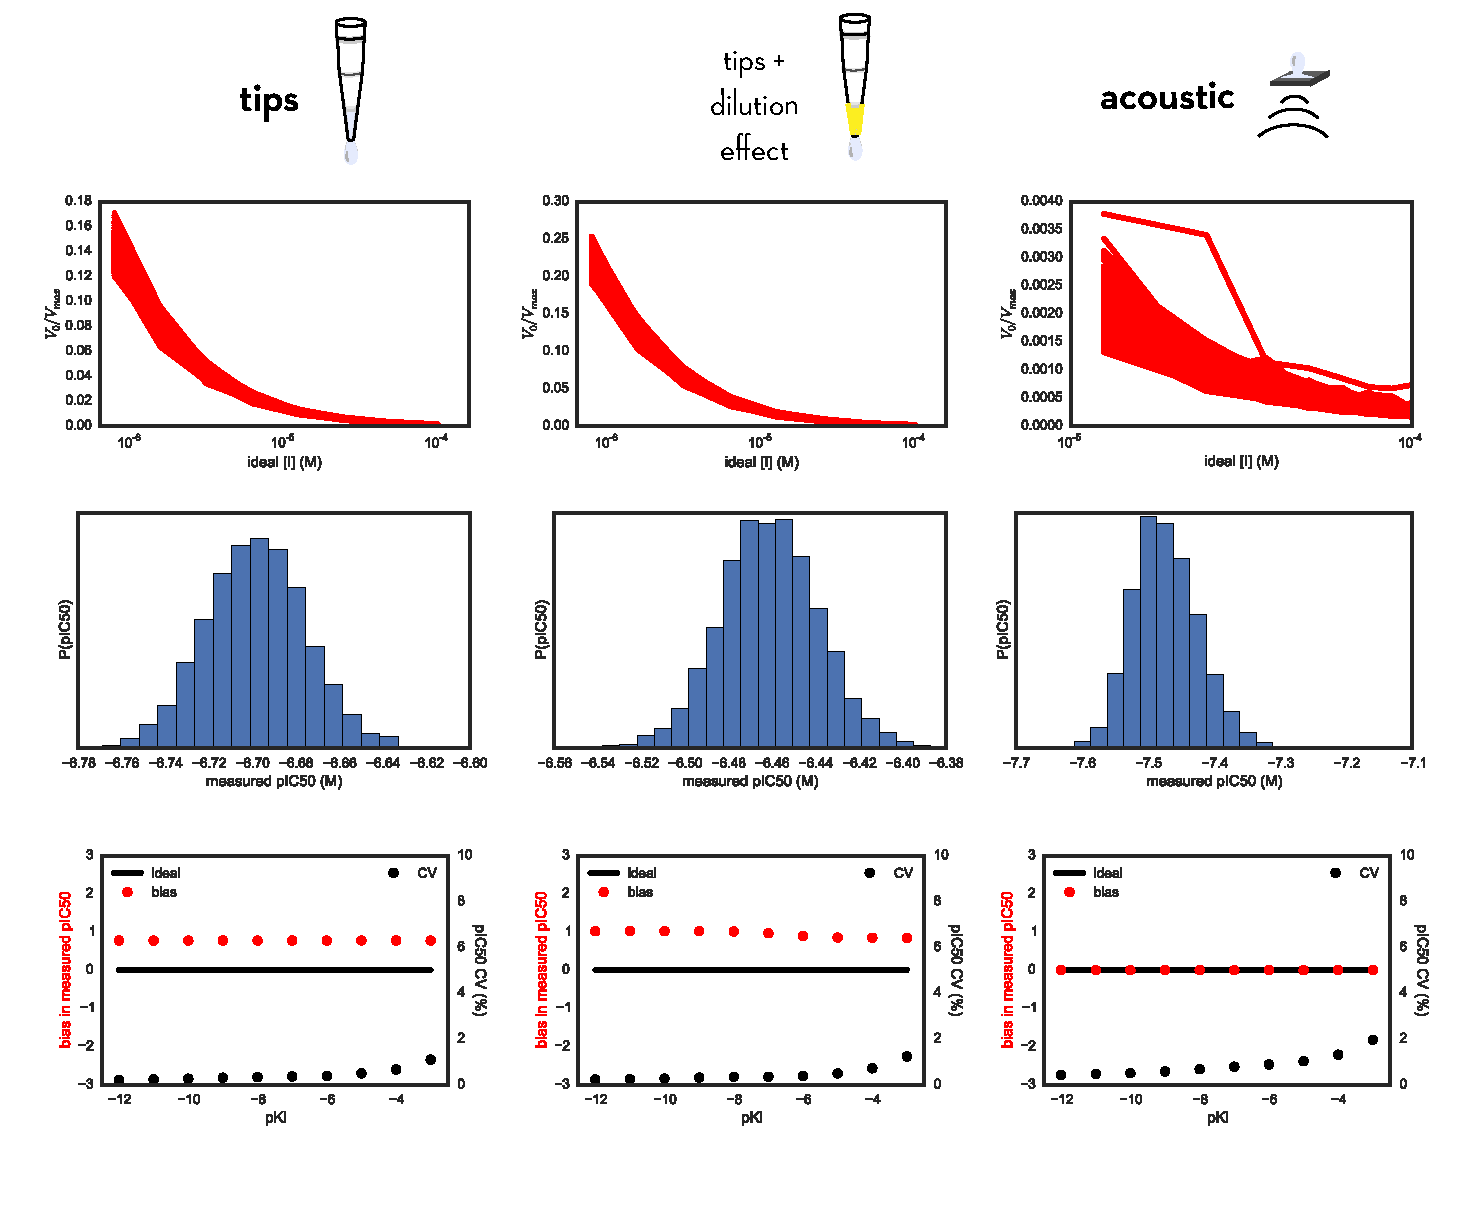
\includegraphics[width=1.0\textwidth]{../figures/acoustic-vs-tips.pdf}
  
  \caption{{\bf Comparing modeled errors in pIC$_{50}$ values from tip-based vs acoustic dispensing.}
  Using our model we can look at the variance in activity measurements as a function of inhibitor concentration $[I]$ (top), which then directly translates into a distribution of measured pIC$_{50}$ values (middle), from which we can find out the bias and variance, or CV, as a function of pKi seen in these assays (bottom). While using acoustic dispensing methods the CV creeps up as a function of pKi, when a known dilution effect is added to the tip-based dispensing, a large bias is easy to spot.
  }
  \label{fig:acoustic-vs-tips}
\end{figure*}

\subsection*{Fitting the assay readout to obtain an IC$_{50}$}

While the IC$_{50}$ reported in the EphB4 assay~\cite{ekins_dispensing_2013,barlaam_novel_2009,barlaam_pyrimidine_2010} in principle represents the stated concentration of inhibitor required to inhibit enzyme activity by half, this value is estimated in practice by numerically fitting a model of inhibition to the measured assay readout (in this case, fluorescence) across the whole range of concentrations measured using a method such as least-squared (the topic of another article in this series~\cite{jones_fitting_2015}).

To mimic the approach used in fitting the assay data, we use a nonlinear least-squares approach (based on the simple {\tt curve\_fit} function from {\tt scipy.optimize}) to fit the competitive inhibition model (Eq.~\ref{equation:competitive-inhibition}) to obtain a $K_i$ and then compute the IC$_{50}$ from this fit value.
We can then use a simple relation between IC$_{50}$ and $K_{i}$ to compute the reported assay readout,
\begin{eqnarray}
\mathrm{IC}_{50} &=& K_{i}\left(1+\frac{[S]}{K_{m}}\right) \label{equation:IC50} .
\end{eqnarray} 
Finally, the reported results are actually $p$IC$_{50}$ values, which are defined by 
\begin{eqnarray}
p\mathrm{IC}_{50} &=& \log_{10} \mathrm{IC}_{50} \label{equation:pIC50}
\end{eqnarray}
Note that no complicated manipulation of these equations is required.
As can be seen in the companion IPython notebook for this article, we simply call {\tt curve\_fit} to obtain a $K_i$ for each experimental replicate, and then store the $p$IC$_{50}$ obtained from use of Eqs.~\ref{equation:IC50} and \ref{equation:pIC50} above.

\subsection*{Imprecision is insufficient to explain the tips vs acoustic discrepancy}

Plotting the inaccuracies and imprecisions and how they differ for tip-based dispensing \emph{vs} direct dispensing is extremely useful, and allows us to better understand the errors in our assay results. 
It is easy to see that simple differences in these values, even when including the compounded error of the dilution series, does not give us much insight into the striking differences seen in the data originally from AstraZeneca ~\cite{ekins_dispensing_2013,barlaam_novel_2009,barlaam_pyrimidine_2010} between tip-based and direct dispensing.

However, if we incorporate the final component of error in tip-based dispensing, the dilution effect, we can see that correcting for this bias in plotting IC$_{50}$ shifts tip-based values more toward direct-dispensing derived values (Figure~\ref{fig:IC50_bias}).

{\color{red}[SMH: I think this section is fine. The brevity gives it power. Feel free to elaborate or move, as you see fit. JDC: This section seems anemic. I think we should either move it entirely to be a part of the Discussion or somehow elaborate on this here.]}

\begin{figure}[tb]
   % 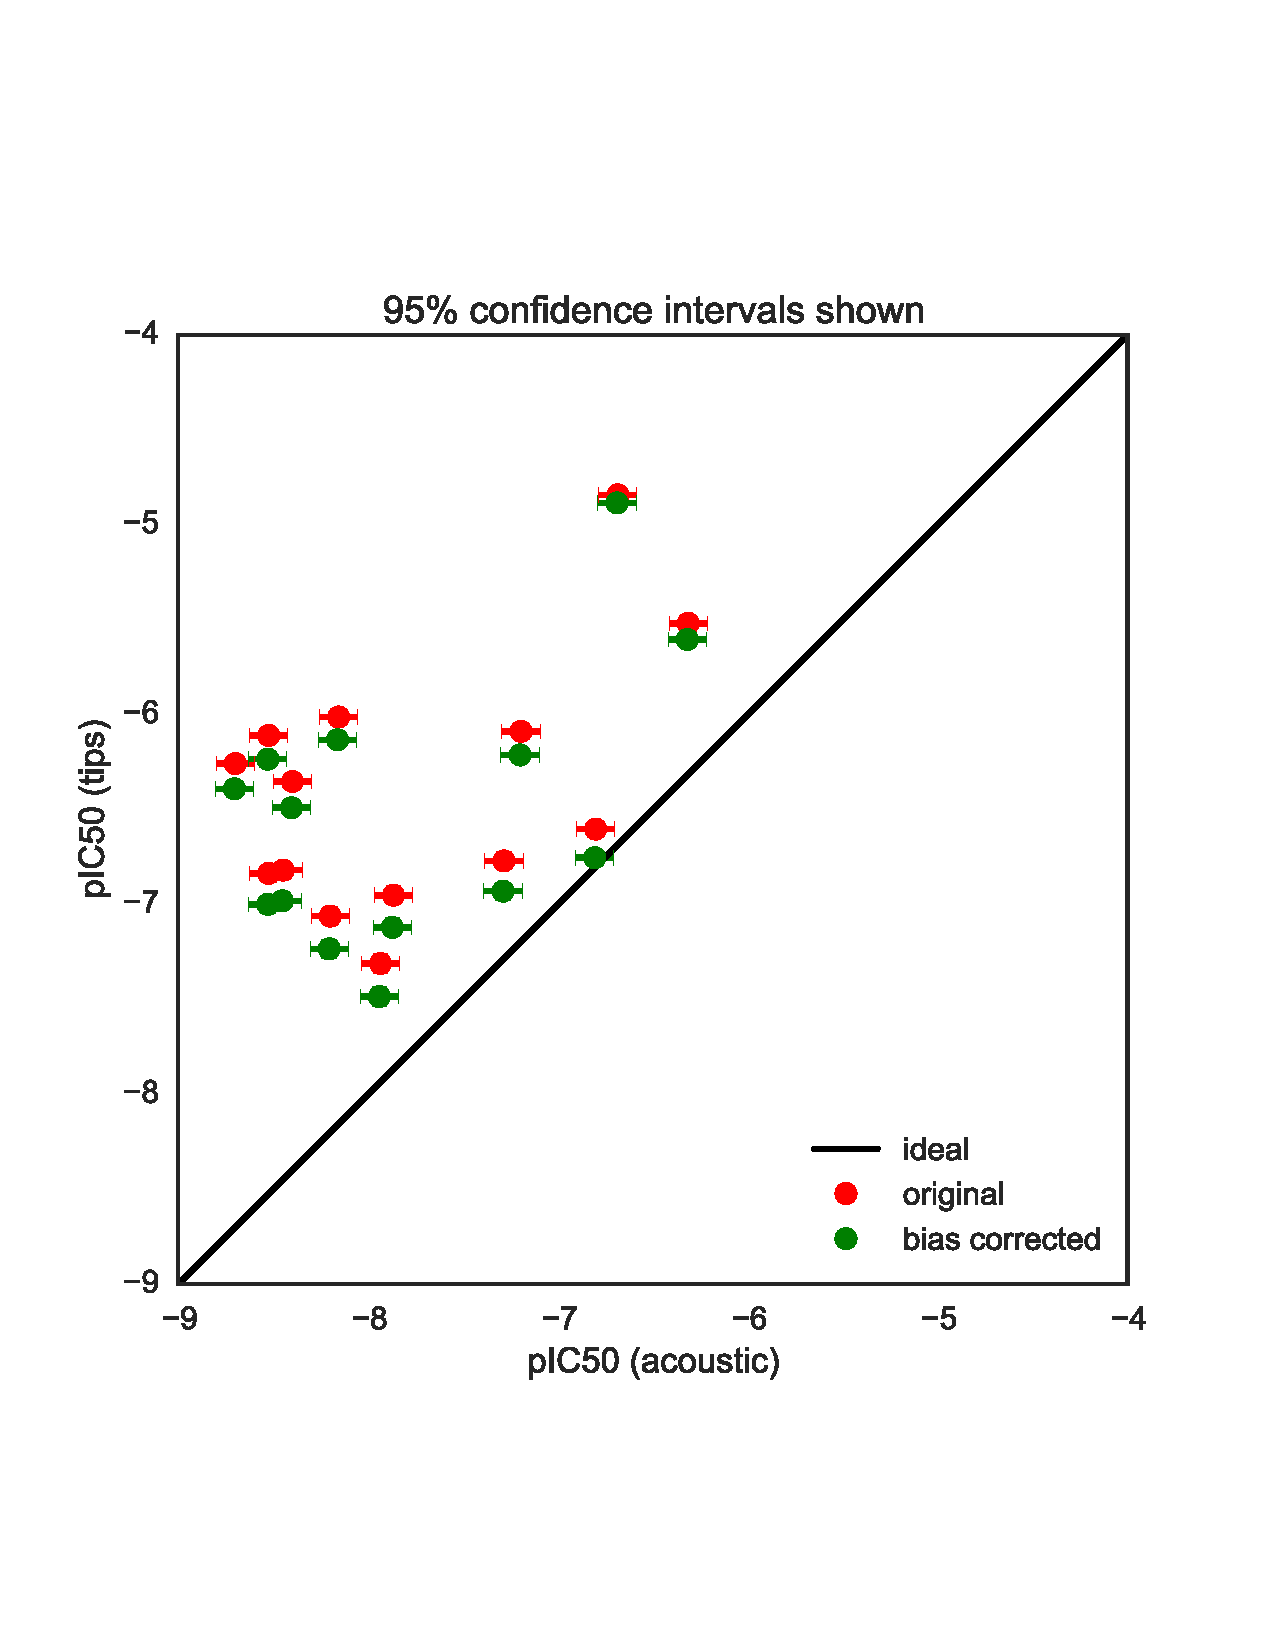
\includegraphics[trim={0 4cm 0 4cm},clip,width=0.5\textwidth]{../figures/compare-pIC50-bias_corrected.pdf}
    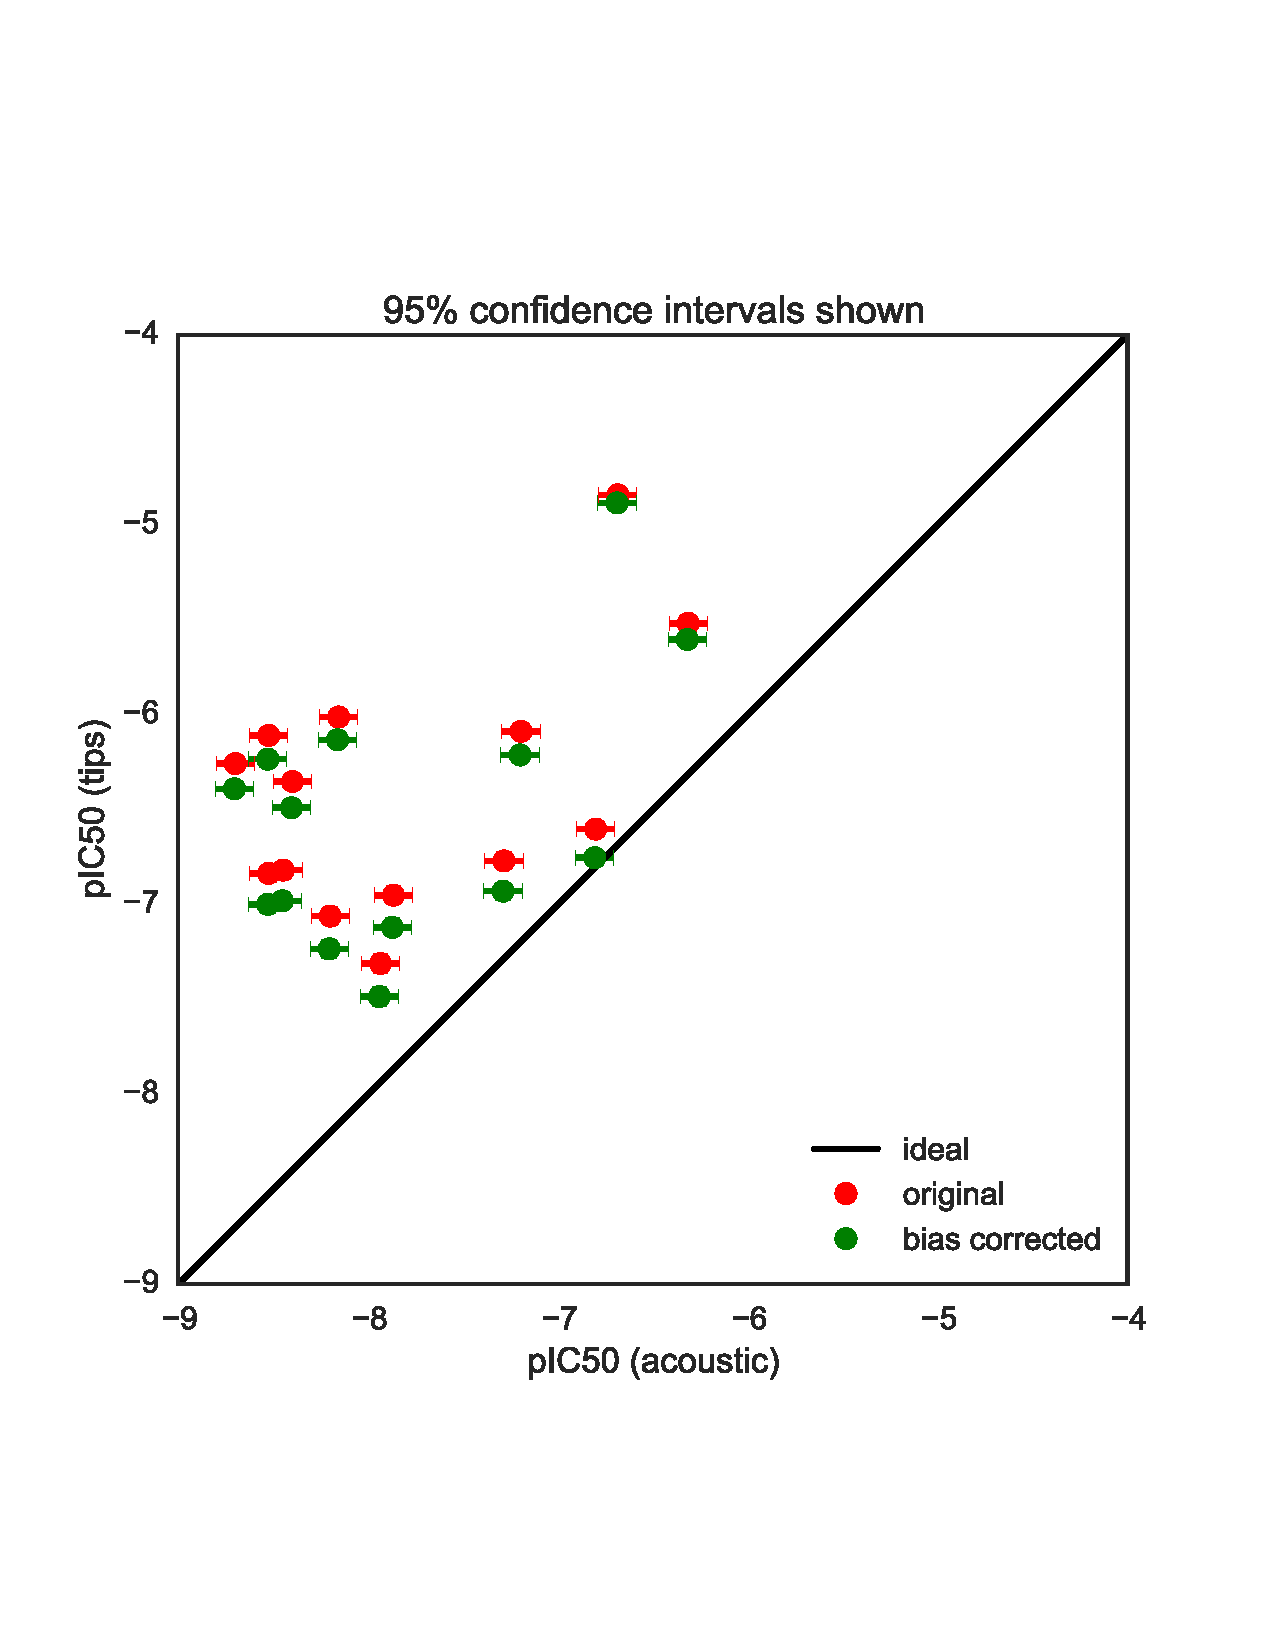
\includegraphics[width=\columnwidth]{../figures/compare-pIC50-bias_corrected.pdf}

  \caption{{\bf Adding bias shifts pIC$_{50}$ values closer to equivalence.}
  Here we see (in red) the original experimental pIC50 values from tips with dilution effect plotted against values from acoustic dispensing with errors bars representing the uncertainty (shown as 95\% confidence intervals) estimated by bootstrapping from our models. 
  Adding in the bias from our bootstrapped models (in green) shifts the experimental pIC$_{50}$ values closer to if tip-based assay and acoustic-based assay measurements resulted in the same final measurement. 
  While this does not entirely explain all discrepancies between the two sets of data, it shifts the root mean square error between the tip-based and acoustic-based dispensing methods from 1.56 to 0.86 pIC50 units.
  The model also demonstrates that (1) the bias induced by the fixed tips explains much of the pIC$_{50}$ shift between the two datasets, and (2) there is still a large degree of variation among the measurements not accounted for by simple imprecision in liquid transfers.
  This demonstrates the power of building simple error models to improve our understanding of experimental data sets.
  }
  \label{fig:IC50_bias}
\end{figure}

%%%%%%%%%%%%%%%%%%%%%%%%%%%%%%%%%%%%%%%%%%%%%%%%%%%%%%%%%%%%%%%%%%%%%%%%%%%%%%%%%%%%%%%%%%%%%%%%%%%%%
% DISCUSSION
%%%%%%%%%%%%%%%%%%%%%%%%%%%%%%%%%%%%%%%%%%%%%%%%%%%%%%%%%%%%%%%%%%%%%%%%%%%%%%%%%%%%%%%%%%%%%%%%%%%%%
\section{Discussion}

Serial dilutions are commonly used in the process of determining biologically and clinically relevant values such as inhibition concentrations (IC$_{ 50}$)  and dissociation constants (K$_{d}$). 
While high-throughput automation methods can improve the reproducibility of these measurements over manual pipetting, even robotic liquid handlers are victim to the accumulation of both random and systematic error.
Since the AstraZeneca dataset~\cite{barlaam_novel_2009,barlaam_pyrimidine_2010} and the related analysis by Ekins et al~\cite{ekins_dispensing_2013}, several studies have posited that acoustic dispensing results in fewer false positives and negatives than tip-based dispensing and that this phenomenon is not isolated to EphB4 receptor inhibitors~\cite{wingfield_impact_2012,olechno_direct_2013,olechno_sound_2013,olechno_improving_2006}. 
Here, we have shed some light on why this might be with some simple modeling, available for extended use through the accompanying iPython notebook.

We have demonstrated how a simple model based on the bootstrap principle, in which nothing more than the manufacturer-provided imprecision and inaccuracy values and a description of the experimental protocol were used to \emph{simulate} virtual replicates of the experiment for a variety of simulated compound affinities allowed us to estimate the imprecision and inaccuracy of measured IC$_{50}$s.
It also identified the difficulty in creating an accurate dilution series using a fix-tip dispenser, with the major contribution to discrepancies in measurements between fixed pipette tip and direct dispensing technologies being the dilution effect. 
In addition to providing some estimate for the random error in measured affinities, the computed bias could even be used to \emph{correct} for the bias introduced by this process after the fact, however we recommend that steps are taken to minimize this bias before the assay is even performed. 
This approach can be a useful general tool for both experimental and computational chemists to understand common sources of error within assays that use dilution series and how to model and correct for them.

This assay is just one example of a large class of assays and this model can be used as a template for other types of experiments relevant to computational modelers.
Instead of simply relying on intuition or historically successful protocol designs, experimentalists could use bootstrap simulation models during assay planning stages to verify that the proposed assay protocol is capable of appropriately discriminating among the properties of the molecules in question given the expected range of IC$_{ 50}$s or K$_{d}$s to be probed, once known errors are accounted for.
Since the model is quantitative, adjusting the parameters in the assay protocol could allow the experimentalist to optimize the protocol to make sure the data is appropriate to the question at hand. 
For example, in our own laboratory, it has informed the decision to use only direct dispensing technologies for our fluorescent ligand-binding assays, in particular the HP D300~\cite{jones_alternative_2013}, whose incorporation into our automated experimental setup will be described in a future work.

Not only is this modeling approach useful for design ahead of time and analysis after the fact of experiments, but it can be extremely useful in determining the right tests and controls to use to be sure errors and biases are properly taken into account in general. If one is not certain about the primary sources of error in an experiment, one is arguably not certain about the results of the experiment in general. 
Understanding these errors, and being certain they are accounted for via clear benchmarks in experimental assays could help ensure the reproducibility of assays in the future, which is currently a topic of great interest. 
Especially with such a wide ranging set of assays that use dilution series, most notably toward the development of proteins and small molecules to study and treat disease, this is a very important category of experiments to understand how to make more clearly reproducible and interpretable.

While here we have illustrated the importance of modeling to the specific case of liquid handling with fixed tips in the context of measuring IC$_{50}$ values for EphB4 inhibitors, there are still large discrepancies that have not been explained, and perhaps variations on this model could explain everything, but perhaps the full explanation comes from parts of the assay yet to be incorporated into this model.
As experiments become more automated and analysis becomes more quantitative, understanding these errors will be increasingly important both for the consumers (computational modelers) and producers (experimentalists) of these data.


%%%%%%%%%%%%%%%%%%%%%%%%%%%%%%%%%%%%%%%%%%%%%%%%%%%%%%%%%%%%%%%%%%%%%%%%%%%%%%%%%%%%%%%%%%%%%%%%%%%%%
% ACKNOWLEDGMENTS
%%%%%%%%%%%%%%%%%%%%%%%%%%%%%%%%%%%%%%%%%%%%%%%%%%%%%%%%%%%%%%%%%%%%%%%%%%%%%%%%%%%%%%%%%%%%%%%%%%%%%
\section{Acknowledgments}
\label{section:acknowledgments}
The authors are grateful to Anthony Nichols (OpenEye) and Martin Stahl (Roche) for organizing the excellent 2013 Computer-Aided Drug Discovery Gordon Research Conference on the topic of ``The Statistics of Drug Discovery'', as well as Terry Stouch, for inspiring many of the ideas in this work.
The authors are especially grateful to Cosma Shalizi for presenting a clear and lucid overview of the bootstrap principle to this audience, and we hope this contribution can further aid readers in the community in employing these principles in their work.
The authors further acknowledge Adrienne Chow and Anthony Lozada of Tecan US for a great deal of assistance in understanding the nature of operation and origin of errors in automated liquid handling equipment.
The authors thank Paul Czodrowski (Merck Darmstadt) for introducing us to IPython notebooks as a means of interactive knowledge transfer.
JDC and SMH acknowledge support from the Sloan Kettering Institute, a Louis V.~Gerstner Young Investigator Award, and NIH grant P30 CA008748.
SE acknowledges Joe Olechno and Antony Williams for extensive discussions on the topic, as well as the many scientists that responded to the various blog posts mentioned herein.

%%%%%%%%%%%%%%%%%%%%%%%%%%%%%%%%%%%%%%%%%%%%%%%%%%%%%%%%%%%%%%%%%%%%%%%%%%%%%%%%%%%%%%%%%%%%%%%%%%%%%
% CONFLICTS OF INTEREST
%%%%%%%%%%%%%%%%%%%%%%%%%%%%%%%%%%%%%%%%%%%%%%%%%%%%%%%%%%%%%%%%%%%%%%%%%%%%%%%%%%%%%%%%%%%%%%%%%%%%%
\section{Conflicts of interest}
\label{section:conflicts-of-interest}

The authors acknowledge no conflicts of interest, but wish to disclose that JDC is on the Scientific Advisory Board of Schr\"{o}dinger and SE is an employee of Collaborative Drug Discovery.

%%%%%%%%%%%%%%%%%%%%%%%%%%%%%%%%%%%%%%%%%%%%%%%%%%%%%%%%%%%%%%%%%%%%%%%%%%%%%%%%%%%%%%%%%%%%%%%%%%%%%%
% BIBLIOGRAPHY
%%%%%%%%%%%%%%%%%%%%%%%%%%%%%%%%%%%%%%%%%%%%%%%%%%%%%%%%%%%%%%%%%%%%%%%%%%%%%%%%%%%%%%%%%%%%%%%%%%%%%%

\bibliographystyle{prsty} 
\bibliography{dispensing-errors.bib}


\end{document}
